% Für Bindekorrektur als optionales Argument "BCORfaktormitmaßeinheit", dann
% sieht auch Option "twoside" vernünftig aus
% Näheres zu "scrartcl" bzw. "scrreprt" und "scrbook" siehe KOMA-Skript Doku
\documentclass[12pt,a4paper,titlepage,headinclude,bibtotoc]{scrartcl}


%---- Allgemeine Layout Einstellungen ------------------------------------------

% Für Kopf und Fußzeilen, siehe auch KOMA-Skript Doku
\usepackage[komastyle]{scrpage2}
\pagestyle{scrheadings}
\automark[section]{chapter}
\setheadsepline{0.5pt}[\color{black}]

%keine Einrückung
\parindent0pt

%Einstellungen für Figuren- und Tabellenbeschriftungen
\setkomafont{captionlabel}{\sffamily\bfseries}
\setcapindent{0em}

\usepackage{caption}

%---- Weitere Pakete -----------------------------------------------------------
% Die Pakete sind alle in der TeX Live Distribution enthalten. Wichtige Adressen
% www.ctan.org, www.dante.de

% Sprachunterstützung
\usepackage[ngerman]{babel}

% Benutzung von Umlauten direkt im Text
% entweder "latin1" oder "utf8"
\usepackage[utf8]{inputenc}

% Pakete mit Mathesymbolen und zur Beseitigung von Schwächen der Mathe-Umgebung
\usepackage{latexsym,exscale,amssymb,amsmath}

% Weitere Symbole
\usepackage[nointegrals]{wasysym}
\usepackage{eurosym}

% Anderes Literaturverzeichnisformat
%\usepackage[square,sort&compress]{natbib}

% Für Farbe
\usepackage{color}

% Zur Graphikausgabe
%Beipiel: \includegraphics[width=\textwidth]{grafik.png}
\usepackage{graphicx}

% Text umfließt Graphiken und Tabellen
% Beispiel:
% \begin{wrapfigure}[Zeilenanzahl]{"l" oder "r"}{breite}
%   \centering
%   \includegraphics[width=...]{grafik}
%   \caption{Beschriftung} 
%   \label{fig:grafik}
% \end{wrapfigure}
\usepackage{wrapfig}

% Mehrere Abbildungen nebeneinander
% Beispiel:
% \begin{figure}[htb]
%   \centering
%   \subfigure[Beschriftung 1\label{fig:label1}]
%   {\includegraphics[width=0.49\textwidth]{grafik1}}
%   \hfill
%   \subfigure[Beschriftung 2\label{fig:label2}]
%   {\includegraphics[width=0.49\textwidth]{grafik2}}
%   \caption{Beschriftung allgemein}
%   \label{fig:label-gesamt}
% \end{figure}
\usepackage{subfigure}
\usepackage{adjustbox}

% Caption neben Abbildung
% Beispiel:
% \sidecaptionvpos{figure}{"c" oder "t" oder "b"}
% \begin{SCfigure}[rel. Breite (normalerweise = 1)][hbt]
%   \centering
%   \includegraphics[width=0.5\textwidth]{grafik.png}
%   \caption{Beschreibung}
%   \label{fig:}
% \end{SCfigure}
\usepackage{sidecap}

% Befehl für "Entspricht"-Zeichen
\newcommand{\corresponds}{\ensuremath{\mathrel{\widehat{=}}}}

%Für chemische Formeln (von www.dante.de)
%% Anpassung an LaTeX(2e) von Bernd Raichle
\makeatletter
\DeclareRobustCommand{\chemical}[1]{%
  {\(\m@th
   \edef\resetfontdimens{\noexpand\)%
       \fontdimen16\textfont2=\the\fontdimen16\textfont2
       \fontdimen17\textfont2=\the\fontdimen17\textfont2\relax}%
   \fontdimen16\textfont2=2.7pt \fontdimen17\textfont2=2.7pt
   \mathrm{#1}%
   \resetfontdimens}}
\makeatother

%Si Einheiten
\usepackage{siunitx}

%c++ Code einbinden
\usepackage{listings}
\lstset{numbers=left, numberstyle=\tiny, numbersep=5pt}

%Differential
\newcommand{\dif}{\ensuremath{\mathrm{d}}}

%Boxen,etc.
\usepackage{fancybox}
\usepackage{empheq}

%Fußnoten auf gleiche Seite
\interfootnotelinepenalty=1000

%Dateien aus Unterverzeichnissen
\usepackage{import}

%Bibliography \bibliography{literatur} und \cite{gerthsen}
%\usepackage{cite}
\usepackage{babelbib}
\selectbiblanguage{ngerman}

\usepackage{eurosym}

\begin{document}

\begin{titlepage}
\centering
\textsc{\Large Anfängerpraktikum der Fakultät für
  Physik,\\[1.5ex] Universität Göttingen}

\vspace*{4.2cm}

\rule{\textwidth}{1pt}\\[0.5cm]
{\huge \bfseries
  Der Transformator\\[1.5ex]
  Protokoll:}\\[0.5cm]
\rule{\textwidth}{1pt}

\vspace*{3.0cm}

\begin{Large}
\begin{tabular}{ll}
Praktikant:
 	&  Felix Kurtz\\
 	&  Michael Lohmann\\

  E-Mail: 
	&  felix.kurtz@stud.uni-goettingen.de\\
	& m.lohmann@stud.uni-goettingen.de\\

 Betreuer: & Björn Klaas\\
 Versuchsdatum: & 10.09.2014\\
\end{tabular}
\end{Large}

\vspace*{0.8cm}

\begin{Large}
\fbox{
  \begin{minipage}[t][2.5cm][t]{6cm} 
    Testat:
  \end{minipage}
}
\end{Large}

\end{titlepage}

\tableofcontents

\newpage

\section{Einleitung}
\label{sec:einleitung}
Im Alltag werden immer wieder \textit{Transformatoren} benötigt, um Spannungen oder elektrische Ströme zu vergrößern/verkleinern.
So wird elektrische Energie über große Distanzen mittels \textit{Hochspannungsleitungen} übertragen, um Verluste zu minimieren.
Dabei werden Spannungen jenseits der 10kV verwendet.
Bei einer Steckdose im Haushalt beträgt die Spannung jedoch nur 230V.\\
In diesem Versuch soll die Funktionsweise eines Transformators betrachtet werden.
Dabei wird auch der \textit{belastete} Transformator untersucht.

\section{Theorie}
\label{sec:theorie}
In der folgenden Abbildung \ref{fig:TrafoSchema} sind die grundlegenden Bestandteile eines Transformators zu sehen.
Dabei ist $U_1$ die Spannung, $I_1$ die Stromstärke sowie die $N_1$ Windungszahl der \textit{Primärspule}.
Analog dazu ist auf der Ausgangsseite die \textit{Sekundärspule}.
\begin{figure}[!htb]
	\centering
	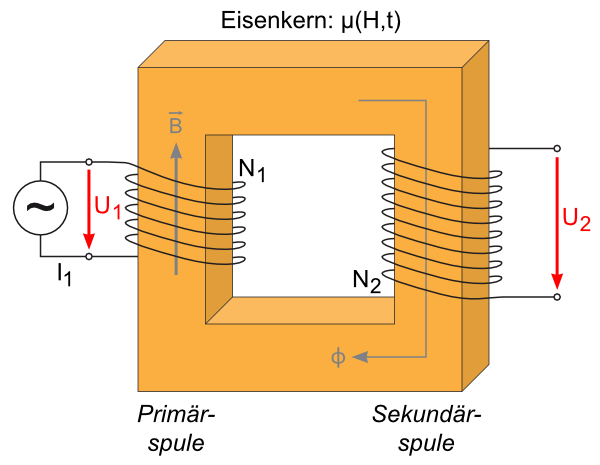
\includegraphics[scale=0.75]{TrafoSchema.png}
	\caption{Schema eines Transformators \cite[Datum: 01.09.2014]{LP16}}
	\label{fig:TrafoSchema}
\end{figure}

\subsection{Unbelasteter Transformator}
Ist der Sekundärkreis nicht geschlossen, spricht man von einem unbelasteten Transformator.
Außerdem liege an der Primärspule eine Wechselspannung $U_1$ an.
Durch den Eisenkern ist der von der Primärspule erzeugte magnetische Fluss durch diese genauso groß wie durch die Sekundärspule.
Mit dem Induktionsgesetz folgt (vgl. \cite[S.432]{gerthsen})
\begin{align*}
	U_1&=N_1 \dot{\Phi} \\
	U_2&=-N_2\dot{\Phi}=-\frac{N_2}{N_1}U_1
\end{align*}

Man erkennt, dass aufgrund der Lenzschen Regel die Spannungen um $180^\circ$ phasenverschoben sind.
Da Primärstrom und -spannung $90^\circ$ phasenverschoben sind, wird in diesem Fall auch keine Energie umgesetzt.

\subsection{Belasteter Transformator}
Wirkleistung
\begin{align}
	P_\text{wirk}=UI\cdot\cos\phi
\end{align}

Verlustleistung
\begin{align}
	P_\text{verlust}=UI\cdot\sin\phi
\end{align}

Phasenverschiebung
\begin{align}
	\tan\phi=\frac{I_0 \sin\phi_0}{I_1+I_0\cos\phi_0}
	\label{eq:phase_theo}
\end{align}
mit $I_2=u\cdot I_1$

Bei einem \textit{idealen} Transformator mit dem Übersetzungsverhältnis $u$ gilt also folgendes:
\begin{align}
	u=\frac{N_1}{N_2}=\frac{U_1}{U_2}=\frac{I_2}{I_1}
	\label{eq:u}  
\end{align}

\subsection{Methoden, um die Phasenverschiebung zu berechnen}
\subsubsection{Lissajous-Figuren}
Um die Phasenverschiebung $\varphi$ zwischen zwei Schwingungen gleicher Frequenz $\omega$ zu bestimmen, trägt man die sich so ergebende Kurve auf:
\begin{align*}
	x(t)&=a\sin(\omega t)\\
	y(t)&=b\sin(\omega t + \varphi)
\end{align*}
Der Schnittpunkt mit der x-Achse bezeichnen wir mit $x_0$, den mit der y-Achse mit $y_0$.
Betrachtet man nun $x=0$, so folgt $\omega t=0$ oder $\omega t=\pi$, also $y_0=b \sin(\varphi)$.
Analog gilt für $y=0:\;x_0=a\sin(\varphi)$.
Also kann so $\varphi$ berechnet werden:
\begin{align}
	\varphi=\arcsin\frac{x_0}{a}=\arcsin\frac{y_0}{b}
	\label{eq:lissajous}
\end{align}
\subsubsection{Zeigerdiagramm}
\begin{figure}[!htb]
	\centering
	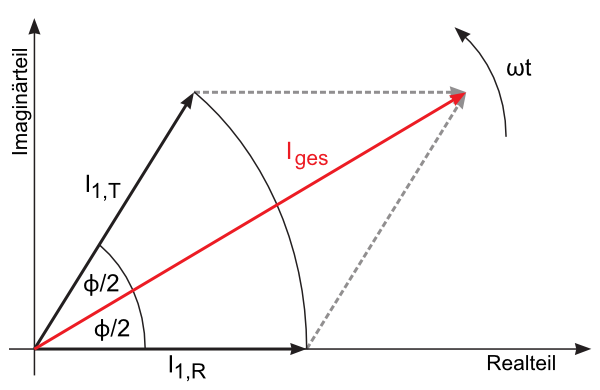
\includegraphics[scale=0.8]{Zeigerdiagramm.png}
	\caption{zugehöriges Zeigerdiagramm \cite[Datum: 01.09.2014]{LP16}}
\end{figure}
\begin{align}
	\cos(\phi/2)=\frac{I_\text{ges}}{2I_1}
	\label{eq:zeigerdiagramm}
\end{align}

\section{Durchführung}
\label{sec:durchfuehrung}
\begin{figure}[!htb]
	\centering	
	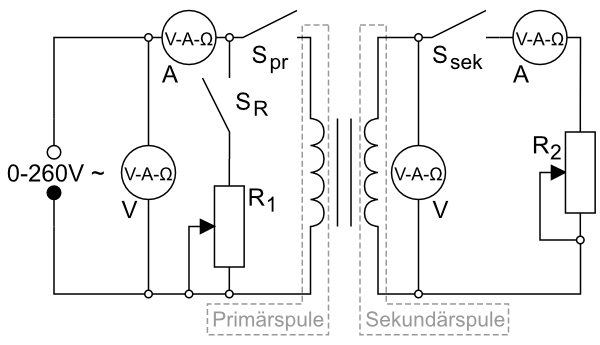
\includegraphics[scale=1.0]{TrafoSchaltung.png}
	\caption{Schaltplan des Versuchaufbaus \cite[Datum: 01.09.2014]{LP16}}
	\label{fig:Schaltung}
\end{figure}
Zuerst wird im \textbf{unbelasteten Fall} (Sekundärkreis nicht geschlossen) $U_1$ in Abhängigkeit von $I_1$.
Da hier keine Widerstände in Betrieb sind, erfolgt die Regelung des Stroms über die Wechselspannungsquelle.
Man nimmt mindestens 20 Werte auf, auch welche bei hohen Spannungen.
Jetzt wird $U_2(U_1)$ gemessen.
Nach Tauschen der Anschlüsse ist die andere Spule Primärspule und man misst wieder die Spannung der Sekundärspule (jetzt $U_1$) in Abhängigkeit der Primärspannung.
Dabei sollte $U_2\leq 20$V sein.\\
Nachdem die Anschlüsse wieder zurück getauscht wurden, wird nun der \textbf{belastete Transformator} gemessen.
Dazu wird der Sekundärkreis geschlossen.
Man achte darauf, dass die Spannung immer vor Öffnen und Schließen eines Schalters auf Null heruntergefahren wird, da sonst hohe Induktionsströme auftreten und diese die Sicherungen der Messgeräte zerstören.
Noch ist $R_1$ nicht geschaltet und an Spule 1 liegt eine Spannung von 200 V an.
Mit dem Schiebewiderstand $R_2$ wird der Sekundärstrom $I_2$ auf 1 A geregelt und der zugehörige Primärstrom $I_1$ notiert.
Nun wird der Widerstand $R_1$ anstelle des Transformator in den Primärkreis geschaltet und so verstellt, dass der nun fließende Strom $I_R$ gleich dem zuvor notierten Wert $I_1$ ist.
Danach wird die Primärspule parallel zum Schiebewiderstand geschaltet, und der Gesamtstrom $I_\text{ges}$ bei gleichem Sekundärstrom $I_2$ wie zuvor gemessen.
Die ganze Messung wird für die Spulenströme 2, 3, 4, und 5 A durchgeführt sowie für 0 A.
Bei letzterer Messung wird der Sekundärkreis geöffnet.\\
Die Phasenverschiebung zwischen Primärspannung und -strom wird mit dem Oszilloskop beobachtet und mit dem zugehörigen Drucker zur weiteren Auswertung ausgedruckt.
Dabei wird die Primärspannung über den Tastkopf (10x) an Channel 1 des Oszilloskops gelegt, während der Strom an Channel 2 anliegt.
Dabei wird die \emph{Stromzange} verwendet.
Außerdem ist $R_1$ nicht im Primärkreis geschaltet.\\
Nun schaltet man das Oszilloskop in den \emph{x-y-Mode} und beobachtet die Änderungen der Kurve bei Veränderung der Last, also den gleichen Strömen $I_2$ wie zuvor.
Die entsprechenden Ergebnisse werden wieder ausgedruckt.

\section{Auswertung}
\label{sec:auswertung}
\subsection{Spannungsquelle}
In Abbildung \ref{fig:UI} ist die Primärspannung gegen den Primärstrom beim unbelasteten Transformator aufgetragen.
Bei einem idealen Transformator würde man eine Ursprungsgerade erwarten.
Dies ist hier jedoch nur bis etwa 150 mA richtig.
Danach steigt die Spannung langsam bis zu einer gewissen \textit{Sättigungsspannung}.
Der Widerstand muss also immer größer werden.
Dies lässt sich damit erklären, dass der Eisenkern gänzlich magnetisiert ist.
\begin{figure}[!htb]
	\centering
	% GNUPLOT: LaTeX picture with Postscript
\begingroup
  \makeatletter
  \providecommand\color[2][]{%
    \GenericError{(gnuplot) \space\space\space\@spaces}{%
      Package color not loaded in conjunction with
      terminal option `colourtext'%
    }{See the gnuplot documentation for explanation.%
    }{Either use 'blacktext' in gnuplot or load the package
      color.sty in LaTeX.}%
    \renewcommand\color[2][]{}%
  }%
  \providecommand\includegraphics[2][]{%
    \GenericError{(gnuplot) \space\space\space\@spaces}{%
      Package graphicx or graphics not loaded%
    }{See the gnuplot documentation for explanation.%
    }{The gnuplot epslatex terminal needs graphicx.sty or graphics.sty.}%
    \renewcommand\includegraphics[2][]{}%
  }%
  \providecommand\rotatebox[2]{#2}%
  \@ifundefined{ifGPcolor}{%
    \newif\ifGPcolor
    \GPcolortrue
  }{}%
  \@ifundefined{ifGPblacktext}{%
    \newif\ifGPblacktext
    \GPblacktexttrue
  }{}%
  % define a \g@addto@macro without @ in the name:
  \let\gplgaddtomacro\g@addto@macro
  % define empty templates for all commands taking text:
  \gdef\gplbacktext{}%
  \gdef\gplfronttext{}%
  \makeatother
  \ifGPblacktext
    % no textcolor at all
    \def\colorrgb#1{}%
    \def\colorgray#1{}%
  \else
    % gray or color?
    \ifGPcolor
      \def\colorrgb#1{\color[rgb]{#1}}%
      \def\colorgray#1{\color[gray]{#1}}%
      \expandafter\def\csname LTw\endcsname{\color{white}}%
      \expandafter\def\csname LTb\endcsname{\color{black}}%
      \expandafter\def\csname LTa\endcsname{\color{black}}%
      \expandafter\def\csname LT0\endcsname{\color[rgb]{1,0,0}}%
      \expandafter\def\csname LT1\endcsname{\color[rgb]{0,1,0}}%
      \expandafter\def\csname LT2\endcsname{\color[rgb]{0,0,1}}%
      \expandafter\def\csname LT3\endcsname{\color[rgb]{1,0,1}}%
      \expandafter\def\csname LT4\endcsname{\color[rgb]{0,1,1}}%
      \expandafter\def\csname LT5\endcsname{\color[rgb]{1,1,0}}%
      \expandafter\def\csname LT6\endcsname{\color[rgb]{0,0,0}}%
      \expandafter\def\csname LT7\endcsname{\color[rgb]{1,0.3,0}}%
      \expandafter\def\csname LT8\endcsname{\color[rgb]{0.5,0.5,0.5}}%
    \else
      % gray
      \def\colorrgb#1{\color{black}}%
      \def\colorgray#1{\color[gray]{#1}}%
      \expandafter\def\csname LTw\endcsname{\color{white}}%
      \expandafter\def\csname LTb\endcsname{\color{black}}%
      \expandafter\def\csname LTa\endcsname{\color{black}}%
      \expandafter\def\csname LT0\endcsname{\color{black}}%
      \expandafter\def\csname LT1\endcsname{\color{black}}%
      \expandafter\def\csname LT2\endcsname{\color{black}}%
      \expandafter\def\csname LT3\endcsname{\color{black}}%
      \expandafter\def\csname LT4\endcsname{\color{black}}%
      \expandafter\def\csname LT5\endcsname{\color{black}}%
      \expandafter\def\csname LT6\endcsname{\color{black}}%
      \expandafter\def\csname LT7\endcsname{\color{black}}%
      \expandafter\def\csname LT8\endcsname{\color{black}}%
    \fi
  \fi
  \setlength{\unitlength}{0.0500bp}%
  \begin{picture}(7200.00,5040.00)%
    \gplgaddtomacro\gplbacktext{%
      \csname LTb\endcsname%
      \put(946,704){\makebox(0,0)[r]{\strut{} 0}}%
      \put(946,1383){\makebox(0,0)[r]{\strut{} 50}}%
      \put(946,2061){\makebox(0,0)[r]{\strut{} 100}}%
      \put(946,2740){\makebox(0,0)[r]{\strut{} 150}}%
      \put(946,3418){\makebox(0,0)[r]{\strut{} 200}}%
      \put(946,4097){\makebox(0,0)[r]{\strut{} 250}}%
      \put(946,4775){\makebox(0,0)[r]{\strut{} 300}}%
      \put(1078,484){\makebox(0,0){\strut{} 0}}%
      \put(2032,484){\makebox(0,0){\strut{} 100}}%
      \put(2986,484){\makebox(0,0){\strut{} 200}}%
      \put(3941,484){\makebox(0,0){\strut{} 300}}%
      \put(4895,484){\makebox(0,0){\strut{} 400}}%
      \put(5849,484){\makebox(0,0){\strut{} 500}}%
      \put(6803,484){\makebox(0,0){\strut{} 600}}%
      \put(176,2739){\rotatebox{-270}{\makebox(0,0){\strut{}Spannung $U_1$ [V]}}}%
      \put(3940,154){\makebox(0,0){\strut{}Strom $I_1$ [mA]}}%
    }%
    \gplgaddtomacro\gplfronttext{%
      \csname LTb\endcsname%
      \put(2398,4602){\makebox(0,0)[r]{\strut{}Messwerte}}%
    }%
    \gplbacktext
    \put(0,0){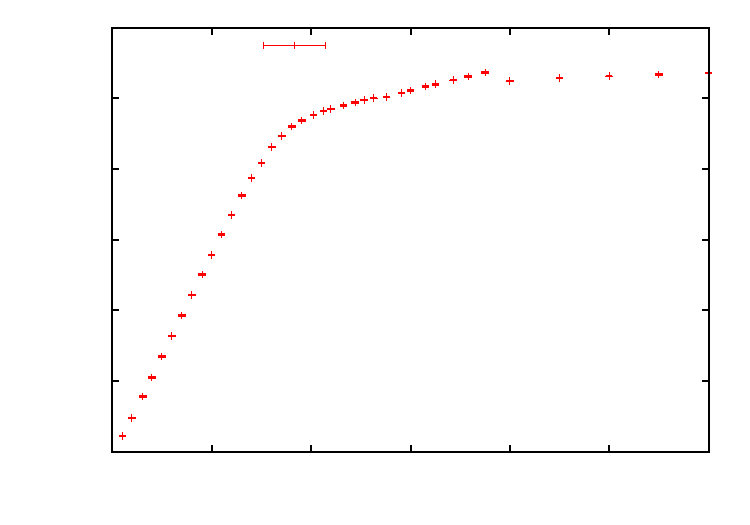
\includegraphics{UI}}%
    \gplfronttext
  \end{picture}%
\endgroup

	\caption{Spannung in Abhängigkeit des Stroms}
	\label{fig:UI}
\end{figure}

\subsection{Übersetzungsverhältnis}
\begin{figure}[!htb]
	\centering
	% GNUPLOT: LaTeX picture with Postscript
\begingroup
  \makeatletter
  \providecommand\color[2][]{%
    \GenericError{(gnuplot) \space\space\space\@spaces}{%
      Package color not loaded in conjunction with
      terminal option `colourtext'%
    }{See the gnuplot documentation for explanation.%
    }{Either use 'blacktext' in gnuplot or load the package
      color.sty in LaTeX.}%
    \renewcommand\color[2][]{}%
  }%
  \providecommand\includegraphics[2][]{%
    \GenericError{(gnuplot) \space\space\space\@spaces}{%
      Package graphicx or graphics not loaded%
    }{See the gnuplot documentation for explanation.%
    }{The gnuplot epslatex terminal needs graphicx.sty or graphics.sty.}%
    \renewcommand\includegraphics[2][]{}%
  }%
  \providecommand\rotatebox[2]{#2}%
  \@ifundefined{ifGPcolor}{%
    \newif\ifGPcolor
    \GPcolortrue
  }{}%
  \@ifundefined{ifGPblacktext}{%
    \newif\ifGPblacktext
    \GPblacktexttrue
  }{}%
  % define a \g@addto@macro without @ in the name:
  \let\gplgaddtomacro\g@addto@macro
  % define empty templates for all commands taking text:
  \gdef\gplbacktext{}%
  \gdef\gplfronttext{}%
  \makeatother
  \ifGPblacktext
    % no textcolor at all
    \def\colorrgb#1{}%
    \def\colorgray#1{}%
  \else
    % gray or color?
    \ifGPcolor
      \def\colorrgb#1{\color[rgb]{#1}}%
      \def\colorgray#1{\color[gray]{#1}}%
      \expandafter\def\csname LTw\endcsname{\color{white}}%
      \expandafter\def\csname LTb\endcsname{\color{black}}%
      \expandafter\def\csname LTa\endcsname{\color{black}}%
      \expandafter\def\csname LT0\endcsname{\color[rgb]{1,0,0}}%
      \expandafter\def\csname LT1\endcsname{\color[rgb]{0,1,0}}%
      \expandafter\def\csname LT2\endcsname{\color[rgb]{0,0,1}}%
      \expandafter\def\csname LT3\endcsname{\color[rgb]{1,0,1}}%
      \expandafter\def\csname LT4\endcsname{\color[rgb]{0,1,1}}%
      \expandafter\def\csname LT5\endcsname{\color[rgb]{1,1,0}}%
      \expandafter\def\csname LT6\endcsname{\color[rgb]{0,0,0}}%
      \expandafter\def\csname LT7\endcsname{\color[rgb]{1,0.3,0}}%
      \expandafter\def\csname LT8\endcsname{\color[rgb]{0.5,0.5,0.5}}%
    \else
      % gray
      \def\colorrgb#1{\color{black}}%
      \def\colorgray#1{\color[gray]{#1}}%
      \expandafter\def\csname LTw\endcsname{\color{white}}%
      \expandafter\def\csname LTb\endcsname{\color{black}}%
      \expandafter\def\csname LTa\endcsname{\color{black}}%
      \expandafter\def\csname LT0\endcsname{\color{black}}%
      \expandafter\def\csname LT1\endcsname{\color{black}}%
      \expandafter\def\csname LT2\endcsname{\color{black}}%
      \expandafter\def\csname LT3\endcsname{\color{black}}%
      \expandafter\def\csname LT4\endcsname{\color{black}}%
      \expandafter\def\csname LT5\endcsname{\color{black}}%
      \expandafter\def\csname LT6\endcsname{\color{black}}%
      \expandafter\def\csname LT7\endcsname{\color{black}}%
      \expandafter\def\csname LT8\endcsname{\color{black}}%
    \fi
  \fi
  \setlength{\unitlength}{0.0500bp}%
  \begin{picture}(7200.00,5040.00)%
    \gplgaddtomacro\gplbacktext{%
      \csname LTb\endcsname%
      \put(1254,704){\makebox(0,0)[r]{\strut{} 0}}%
      \put(1254,1383){\makebox(0,0)[r]{\strut{} 50}}%
      \put(1254,2061){\makebox(0,0)[r]{\strut{} 100}}%
      \put(1254,2740){\makebox(0,0)[r]{\strut{} 150}}%
      \put(1254,3419){\makebox(0,0)[r]{\strut{} 200}}%
      \put(1254,4097){\makebox(0,0)[r]{\strut{} 250}}%
      \put(1254,4776){\makebox(0,0)[r]{\strut{} 300}}%
      \put(1386,484){\makebox(0,0){\strut{} 0}}%
      \put(2500,484){\makebox(0,0){\strut{} 5}}%
      \put(3615,484){\makebox(0,0){\strut{} 10}}%
      \put(4729,484){\makebox(0,0){\strut{} 15}}%
      \put(5844,484){\makebox(0,0){\strut{} 20}}%
      \put(6958,484){\makebox(0,0){\strut{} 25}}%
      \put(484,2740){\rotatebox{90}{\makebox(0,0){\strut{}Spannung $U_1$ [V]}}}%
      \put(4172,154){\makebox(0,0){\strut{}Spannung $U_2$ [V]}}%
    }%
    \gplgaddtomacro\gplfronttext{%
      \csname LTb\endcsname%
      \put(4686,4603){\makebox(0,0)[r]{\strut{}Messwerte $U_2(U_1)$}}%
      \csname LTb\endcsname%
      \put(4686,4383){\makebox(0,0)[r]{\strut{}zugeh. Regressionsgerade}}%
      \csname LTb\endcsname%
      \put(4686,4163){\makebox(0,0)[r]{\strut{}Messwerte $U_1(U_2)$}}%
      \csname LTb\endcsname%
      \put(4686,3943){\makebox(0,0)[r]{\strut{}zugeh. Regressionsgerade}}%
    }%
    \gplbacktext
    \put(0,0){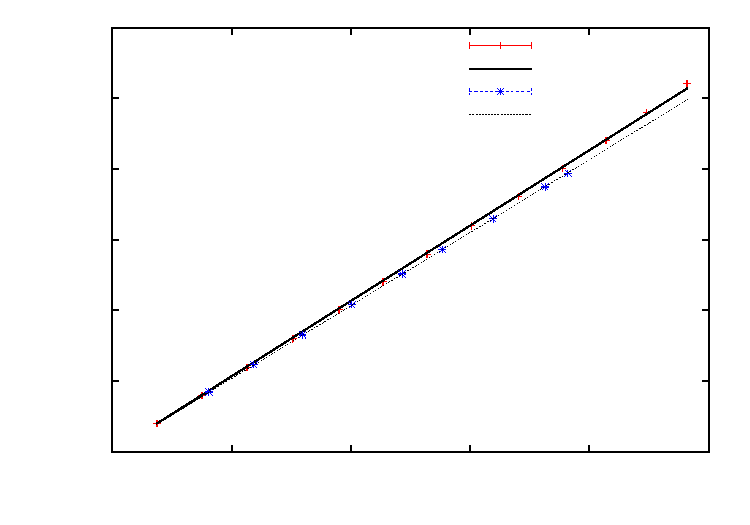
\includegraphics{uebersetzung}}%
    \gplfronttext
  \end{picture}%
\endgroup

	\caption{Abhängigkeiten zwischen Primär- und Sekundärspannung}
	\label{fig:uerbersetzung}
\end{figure}

Trägt man die Primärspannung gegen die Sekundärspannung auf (Abb.\ref{fig:uerbersetzung}), ist die sich ergebende Geradensteigung das Übersetzungsverhältnis $u$.
Dies folgt aus \eqref{eq:u}.
Da wir einmal $U_2$ in Abh. von $U_1$ gemessen haben und das andere Mal $U_1(U_2)$, ergeben sich auch zwei Geraden mit den Steigungen $u=10.663 \pm 0.025$ und $u=10.331 \pm 0.007$.
Der gewichtete Mittelwert beträgt:
\begin{empheq}[box=\shadowbox*]{align}
	u=10.353 \pm 0.007
	\label{res:u}
\end{empheq}


\subsection{Phasenverschiebung zwischen Spannung und Strom}
Um die Phasenverschiebung zu bestimmen, wurden 3 Methoden verwendet:
Zum einen hat das Oszilloskop die Verschiebung im y-t-Mode angezeigt, zum anderen haben wir aus den Ausdrucken der Lissajous-Figuren mithilfe \eqref{eq:lissajous} $\varphi$ bestimmt.
Außerdem haben wir die wichtigen Werte für die Zeigerdiagramm-Methode gemessen.
Mit \eqref{eq:zeigerdiagramm} wurde daraus die Phasenverschiebung berechnet.
All dies ist in der Abbildung \ref{fig:Phase} zu sehen.
Darin wurde auch die Theoriekurve aus \eqref{eq:phase_theo} eingezeichnet.
Hierbei verwenden wir $I_0=0.15\,$A und $\varphi_0=\pi/2$ sowie die zuvor berechnete Übersetzung \eqref{res:u}.
\begin{figure}[!htb]
	\centering
	% GNUPLOT: LaTeX picture with Postscript
\begingroup
  \makeatletter
  \providecommand\color[2][]{%
    \GenericError{(gnuplot) \space\space\space\@spaces}{%
      Package color not loaded in conjunction with
      terminal option `colourtext'%
    }{See the gnuplot documentation for explanation.%
    }{Either use 'blacktext' in gnuplot or load the package
      color.sty in LaTeX.}%
    \renewcommand\color[2][]{}%
  }%
  \providecommand\includegraphics[2][]{%
    \GenericError{(gnuplot) \space\space\space\@spaces}{%
      Package graphicx or graphics not loaded%
    }{See the gnuplot documentation for explanation.%
    }{The gnuplot epslatex terminal needs graphicx.sty or graphics.sty.}%
    \renewcommand\includegraphics[2][]{}%
  }%
  \providecommand\rotatebox[2]{#2}%
  \@ifundefined{ifGPcolor}{%
    \newif\ifGPcolor
    \GPcolortrue
  }{}%
  \@ifundefined{ifGPblacktext}{%
    \newif\ifGPblacktext
    \GPblacktexttrue
  }{}%
  % define a \g@addto@macro without @ in the name:
  \let\gplgaddtomacro\g@addto@macro
  % define empty templates for all commands taking text:
  \gdef\gplbacktext{}%
  \gdef\gplfronttext{}%
  \makeatother
  \ifGPblacktext
    % no textcolor at all
    \def\colorrgb#1{}%
    \def\colorgray#1{}%
  \else
    % gray or color?
    \ifGPcolor
      \def\colorrgb#1{\color[rgb]{#1}}%
      \def\colorgray#1{\color[gray]{#1}}%
      \expandafter\def\csname LTw\endcsname{\color{white}}%
      \expandafter\def\csname LTb\endcsname{\color{black}}%
      \expandafter\def\csname LTa\endcsname{\color{black}}%
      \expandafter\def\csname LT0\endcsname{\color[rgb]{1,0,0}}%
      \expandafter\def\csname LT1\endcsname{\color[rgb]{0,1,0}}%
      \expandafter\def\csname LT2\endcsname{\color[rgb]{0,0,1}}%
      \expandafter\def\csname LT3\endcsname{\color[rgb]{1,0,1}}%
      \expandafter\def\csname LT4\endcsname{\color[rgb]{0,1,1}}%
      \expandafter\def\csname LT5\endcsname{\color[rgb]{1,1,0}}%
      \expandafter\def\csname LT6\endcsname{\color[rgb]{0,0,0}}%
      \expandafter\def\csname LT7\endcsname{\color[rgb]{1,0.3,0}}%
      \expandafter\def\csname LT8\endcsname{\color[rgb]{0.5,0.5,0.5}}%
    \else
      % gray
      \def\colorrgb#1{\color{black}}%
      \def\colorgray#1{\color[gray]{#1}}%
      \expandafter\def\csname LTw\endcsname{\color{white}}%
      \expandafter\def\csname LTb\endcsname{\color{black}}%
      \expandafter\def\csname LTa\endcsname{\color{black}}%
      \expandafter\def\csname LT0\endcsname{\color{black}}%
      \expandafter\def\csname LT1\endcsname{\color{black}}%
      \expandafter\def\csname LT2\endcsname{\color{black}}%
      \expandafter\def\csname LT3\endcsname{\color{black}}%
      \expandafter\def\csname LT4\endcsname{\color{black}}%
      \expandafter\def\csname LT5\endcsname{\color{black}}%
      \expandafter\def\csname LT6\endcsname{\color{black}}%
      \expandafter\def\csname LT7\endcsname{\color{black}}%
      \expandafter\def\csname LT8\endcsname{\color{black}}%
    \fi
  \fi
  \setlength{\unitlength}{0.0500bp}%
  \begin{picture}(7200.00,5040.00)%
    \gplgaddtomacro\gplbacktext{%
      \csname LTb\endcsname%
      \put(946,918){\makebox(0,0)[r]{\strut{} 0}}%
      \put(946,1347){\makebox(0,0)[r]{\strut{} 0.2}}%
      \put(946,1775){\makebox(0,0)[r]{\strut{} 0.4}}%
      \put(946,2204){\makebox(0,0)[r]{\strut{} 0.6}}%
      \put(946,2632){\makebox(0,0)[r]{\strut{} 0.8}}%
      \put(946,3061){\makebox(0,0)[r]{\strut{} 1}}%
      \put(946,3489){\makebox(0,0)[r]{\strut{} 1.2}}%
      \put(946,3918){\makebox(0,0)[r]{\strut{} 1.4}}%
      \put(946,4346){\makebox(0,0)[r]{\strut{} 1.6}}%
      \put(946,4775){\makebox(0,0)[r]{\strut{} 1.8}}%
      \put(1279,484){\makebox(0,0){\strut{} 0}}%
      \put(2283,484){\makebox(0,0){\strut{} 1}}%
      \put(3288,484){\makebox(0,0){\strut{} 2}}%
      \put(4292,484){\makebox(0,0){\strut{} 3}}%
      \put(5296,484){\makebox(0,0){\strut{} 4}}%
      \put(6301,484){\makebox(0,0){\strut{} 5}}%
      \put(176,2739){\rotatebox{-270}{\makebox(0,0){\strut{}Phasenwinkel $\phi$ [rad]}}}%
      \put(3940,154){\makebox(0,0){\strut{}Strom $I_2$ [A]}}%
    }%
    \gplgaddtomacro\gplfronttext{%
      \csname LTb\endcsname%
      \put(5170,4602){\makebox(0,0)[r]{\strut{}Messwerte}}%
      \csname LTb\endcsname%
      \put(5170,4382){\makebox(0,0)[r]{\strut{}Messwerte Oszi}}%
      \csname LTb\endcsname%
      \put(5170,4162){\makebox(0,0)[r]{\strut{}Lissajous}}%
      \csname LTb\endcsname%
      \put(5170,3942){\makebox(0,0)[r]{\strut{}theoretisch erwarteter Verlauf}}%
    }%
    \gplbacktext
    \put(0,0){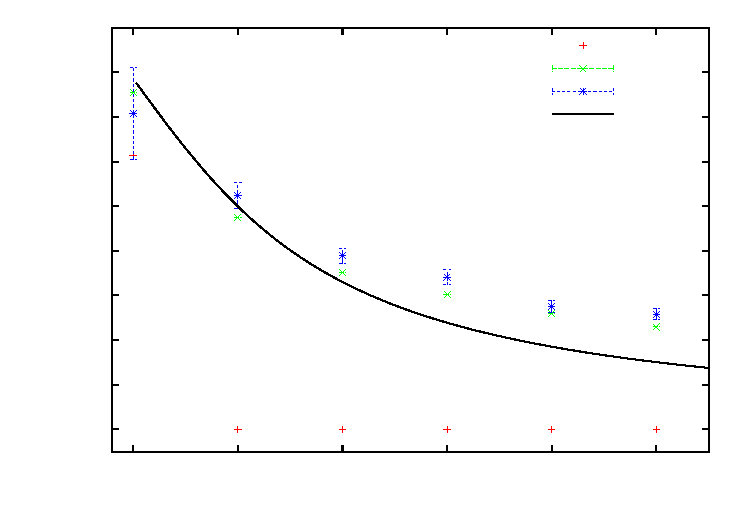
\includegraphics{Phase}}%
    \gplfronttext
  \end{picture}%
\endgroup

	\caption{Phasenverschiebung}
	\label{fig:Phase}
\end{figure}

\subsection{Leistung}
Bei einer Spannung $U=200\,$V und einem Strom $I_2=5\,$A, also $I_1=0.48\,$A ergibt sich mit der oben berechneten Phasenverschiebung $\delta=(0.498 \pm 0.020) \,$rad (gewichteter Mittelwert aus Oszi- und Lissajous-Messung) ergeben sich folgende Wirk- und Verlustleistungen:
\begin{empheq}[box=\shadowbox*]{align*}
	P_\text{wirk}=(84.4 \pm 0.9)\,\si{\watt} \qquad
	P_\text{verlust}=(45.8 \pm 1.7)\,\si{\watt}
\end{empheq}
Aus unseren Transformator-Werten $U=200\,$V und $I_1(I_2=0\,\si{\ampere})=0.11\,$A sowie der Phasenverschiebung $\delta=(1.51 \pm 0.04)\,$rad  ergibt sich eine Leerlauf-Leistung von $(6.1 \pm 3.3)\,$W.
Setzt man für ein Handyladegerät die gleichen Werte an und bezahlt einen Strompreis von $0.25\,$\euro/kWh, bezahlt man folgendes pro Jahr, wenn das  Ladegerät in der Steckdose verbleibt:
\begin{empheq}[box=\shadowbox*]{align*}
	365.2425 \,\frac{\text{d}}{\text{a}}\cdot 24 \,\frac{\text{h}}{\text{d}}\cdot 0.25\,\frac{\text{\euro}}{\text{kWh}}\cdot (6.1 \pm 3.3)\,\si{\watt}=(13.37 \pm 7.24)\,\frac{\text{\euro}}{\text{a}}
\end{empheq}
Von diesem Geld könnte man sich stattdessen ein bis zwei Pizzen bestellen. 

\section{Diskussion}
\label{sec:diskussion}
Die Bestimmung der Phasenverschiebung mittels \textbf{Zeigerdiagramm} lieferte keine brauchbaren Ergebnisse.
So sind zwar in Abb. \ref{fig:Phase} Werte für 1A - 5A zu sehen.
Jedoch wurde hier der arccos aus einer Zahl größer 1 berechnet.
Das Programm \textit{Gnuplot} setzt einen solchen Wert auf 0. 
 fiel uns schon während des Versuches auf, da $I_\text{ges}$ in etwa doppelt so groß war wie $I_1$.
Also wäre die Phasenverschiebung konstant bei 0.
Uns ist jedoch immer noch schleierhaft, warum bei dieser Messung solche Werte gemessen wurden.
Auch die anderen beiden Gruppen hatten das gleiche Phänomen.
Für zukünftige Praktikanten sollte dies untersucht und evtl. behoben werden.
Falls unser Aufbau fehlerhaft war, muss darauf in Zukunft in der Praktikumsanleitung hingewiesen werden.\\

Da das \textbf{Übersetzungsverhältnis} meist ganzzahlig ist, gehen wir bei unserem Ergebnis \eqref{res:u} davon aus, dass das tatsächliche Verhältnis $u=10$ ist.
Somit haben wir eine Abweichung von etwa $3.5\%$.


\bibliography{literatur}
\bibliographystyle{babalpha}

\end{document}
